\documentclass[border=2pt]{standalone}
\usepackage{pgfplots}
\usepgfplotslibrary{colorbrewer}

\begin{document}

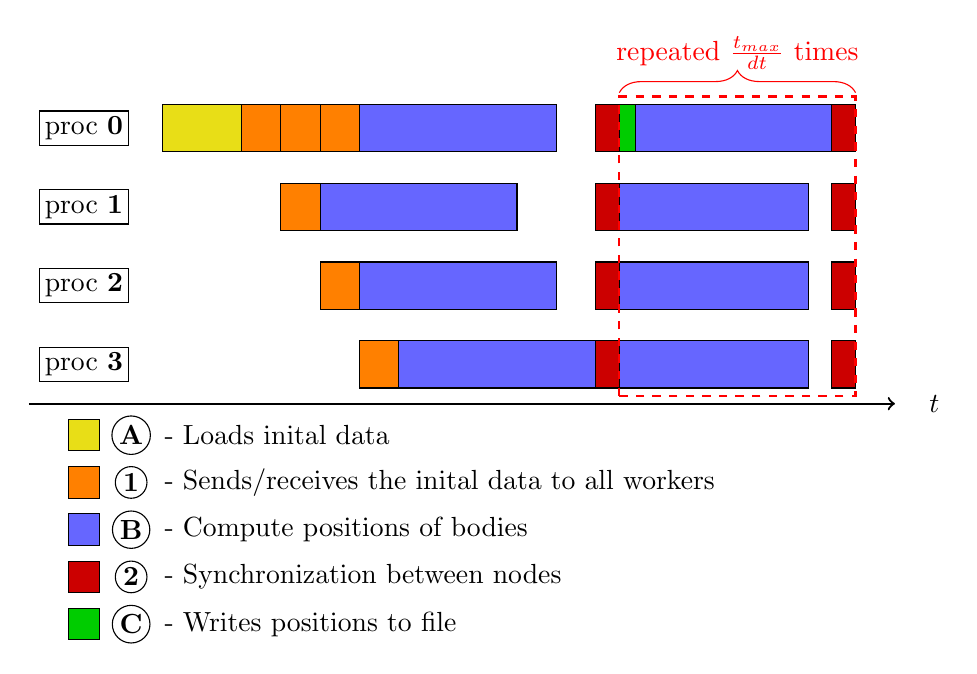
\begin{tikzpicture}  
  \node[draw,rectangle,inner sep=2pt] at (0,0.0) {proc \textbf{0}};
  \node[draw,rectangle,inner sep=2pt] at (0,-1) {proc \textbf{1}};
  \node[draw,rectangle,inner sep=2pt] at (0,-2) {proc \textbf{2}};
  \node[draw,rectangle,inner sep=2pt] at (0,-3) {proc \textbf{3}};
  
  % proc 0
  \filldraw[yellow!90!black, draw = black] (1.0,-0.3) rectangle (2.0,0.3);

  \filldraw[orange, draw=black] (2.0,-0.3) rectangle (2.5,0.3);
  \filldraw[orange, draw=black] (2.5,-0.3) rectangle (3.0,0.3);
  \filldraw[orange, draw=black] (3.0,-0.3) rectangle (3.5,0.3);

  \filldraw[blue!60!white, draw=black] (3.5,-0.3) rectangle (6.0,0.3);
  \filldraw[red!80!black, draw=black] (6.5,-0.3) rectangle (6.8,0.3);
  \filldraw[green!80!black, draw=black] (6.8,-0.3) rectangle (7.0,0.3);

  \filldraw[blue!60!white, draw=black] (7.0,-0.3) rectangle (9.5,0.3);
  \filldraw[red!80!black, draw=black] (9.5,-0.3) rectangle (9.8,0.3);
  % proc 1
  \filldraw[orange, draw=black] (2.5,-1.3) rectangle (3.0,-0.7);
  \filldraw[blue!60!white, draw=black] (3.0,-1.3) rectangle (5.5,-0.7);
  \filldraw[red!80!black, draw=black] (6.5,-1.3) rectangle (6.8,-0.7);

  \filldraw[blue!60!white, draw=black] (6.8,-1.3) rectangle (9.2,-0.7);
  \filldraw[red!80!black, draw=black] (9.5,-1.3) rectangle (9.8,-0.7);
  % proc 2
  \filldraw[orange, draw=black] (3.0,-2.3) rectangle (3.5,-1.7);
  \filldraw[blue!60!white, draw=black] (3.5,-2.3) rectangle (6.0,-1.7);
  \filldraw[red!80!black, draw=black] (6.5,-2.3) rectangle (6.8,-1.7);

  \filldraw[blue!60!white, draw=black] (6.8,-2.3) rectangle (9.2,-1.7);
  \filldraw[red!80!black, draw=black] (9.5,-2.3) rectangle (9.8,-1.7);
  % proc 3
  \filldraw[orange, draw=black] (3.5,-3.3) rectangle (4.0,-2.7);
  \filldraw[blue!60!white, draw=black](4.0,-3.3) rectangle (6.5,-2.7);
  \filldraw[red!80!black, draw=black] (6.5, -3.3) rectangle (6.8, -2.7);

  \filldraw[blue!60!white, draw=black] (6.8,-3.3) rectangle (9.2,-2.7);
  \filldraw[red!80!black, draw=black] (9.5,-3.3) rectangle (9.8, -2.7);

  \draw[red, dashed, thick] (6.8,-3.4) rectangle (9.8, 0.4);
  \draw [red,decorate,decoration={brace,amplitude=8pt}] (6.8, 0.45) -- node [pos=0.5, midway, yshift=0.5cm] {repeated $\frac{t_{max}}{dt}$ times} (9.8,0.45);

  \draw[->, thick] (-0.7, -3.5) -- (10.3,-3.5) node[xshift=0.5cm] {$t$};
  % legend
  \filldraw[yellow!90!black, draw = black] (-0.2,-4.1) rectangle (0.2,-3.7);
  \filldraw[orange, draw=black] (-0.2,-4.7) rectangle (0.2,-4.3);
  \filldraw[blue!60!white, draw=black] (-0.2,-5.3) rectangle (0.2,-4.9);
  \filldraw[red!80!black, draw=black] (-0.2,-5.9) rectangle (0.2,-5.5);
  \filldraw[green!80!black, draw=black] (-0.2,-6.5) rectangle (0.2,-6.1);
  
  \node[draw,circle,inner sep=1pt] at (0.6,-3.9) {\textbf{A}};
  \node[draw,circle,inner sep=1pt] at (0.6,-4.5) {\textbf{1}};
  \node[draw,circle,inner sep=1pt] at (0.6,-5.1) {\textbf{B}};
  \node[draw,circle,inner sep=1pt] at (0.6,-5.7) {\textbf{2}};
  \node[draw,circle,inner sep=1pt] at (0.6,-6.3) {\textbf{C}};

  \node[right] at (0.9,-3.9) {- Loads inital data};
  \node[right] at (0.9,-4.5) {- Sends/receives the inital data to all workers};
  \node[right] at (0.9,-5.1) {- Compute positions of bodies};
  \node[right] at (0.9,-5.7) {- Synchronization between nodes};
  \node[right] at (0.9,-6.3) {- Writes positions to file};

\end{tikzpicture}
\end{document}
